% ##################################################################################################################
\chapter{Caracas: Scenario}
\label{ch:caracas}
\hfill \textbf{Authors:} Walter J. Hernández B., Héctor E. Navarro U.
%\editdone{This text has undergone the professional edit. Please no grammatical changes anymore! They are most-probably wrong.}
% ##################################################################################################################

Being the capital of the country, Caracas is the largest city of Venezuela and one in particular, where vehicle traffic is quite serious. With a daily estimated circulation of 1.5\,million units, this number represents three times the load originally estimated for the city's growth. %One of the current main issues for planning is 
Despite the lack of official statistics, it is possible to estimate the amount of traffic of Caracas using other nation wide figures, such as the \emph{Time Travel Index} employed by the \citet{fhwa2013}, which allows to surmise an approx. 50\,\% longer than \textit{free-flow travel} to move around the inner circles of the city and 75\,\% around the metropolitan areas. This is in stark contrast to an average city in the US, which normally does not go beyond 35\,\% in the worst case.

Apart from the obvious budget-related deficits that these delays cause to the working force productivity for companies and organizations, the country itself loses an estimated \$2.1\,billion per year. This is only including the precious subsidies that have helped to maintain the country's world lowest prices of gas for decades (\citet{wilson2008}), and still, \$1\,billion could be saved by reducing the average circulation time in just 30\,minutes. Plus a significant reduction on \gls{co2} emissions, that in turn would help to meet greenhouse emission targets for the country.

Several initiatives have been put in place in recent years to cope with the increased traffic in Caracas:

\begin{itemize}\styleItemize
\item \gls{hov} lanes (\citet{turnbull1990}), implemented in a \textit{contraflow} fashion to increase traffic flow on central roads and highways.

\item Bus lanes for rapid bus trips and bicycle lanes, to stimulate the use of alternative means of transport.

\item Shifting the sign-in hour of jobs to non-peak times and also increasing the number of working hours from home of certain types of jobs, to cut back vehicle use and costs to public transport in general.
\end{itemize}

In addition to the these measures, some other mechanisms could be implemented, such as weekday circulation restrictions (\eg based on the license plate number) and smart traffic lights. Whatever the case, but especially in the case of smart traffic devices and planning of special lanes, careful study and simulation of traffic patterns must be taken. Considering this latter aspect, a software tool was envisioned with the following objectives:

\begin{itemize}
 \item To visually engage the creation and editing of traffic networks on \gls{matsim} format, and also the assignment of validation points to the network.

\item To visually engage the study of the results from simulations, especially the traffic volumes assigned to roads.

\item To translate data obtained in \gls{od} format for input to \gls{matsim}.

\item To run the simulations and validate outputs in order to calibrate the parameters involved.
\end{itemize}

The tool was tested with real data traffic in an area of Caracas named ``Los Cortijos'' (Figure~\ref{fig:caracas1left}), one of the most transited zones on the east side of the city. The simulation model falls under the \emph{microscopic} category made by \citet{gartner2001}, since only individuals elements are taken into account (i.e, vehicles).

 %------------
\createfigure%
{An area of ``Los Cortijos'' in Caracas, Venezuela.}%
{An area of ``Los Cortijos'' in Caracas, Venezuela.}%
{\label{fig:caracas1}}%
{%
 \createsubfigure%
 {Snapshot obtained from \gls{osm}.}
 {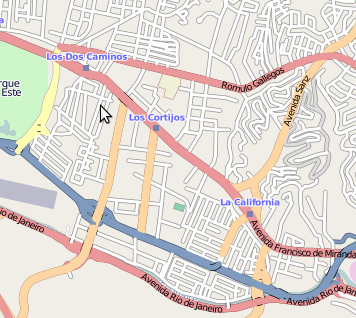
\includegraphics[width=0.35\textwidth, angle=0]{./scenarios/figures/caracas0.png}}
 {\label{fig:caracas1left}}
\createsubfigure%
 {Three snapshots of a simulation ran in \gls{matsim} between 6:00 and 6:30 am, depicting the increasing traffic in the zone}
 {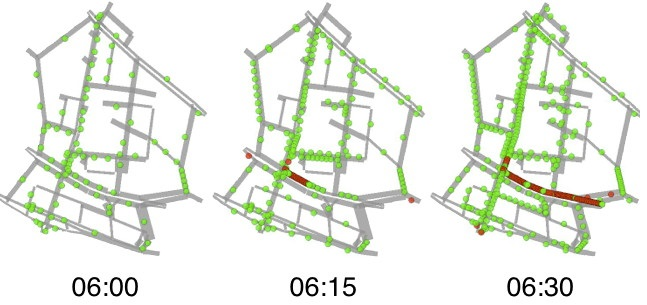
\includegraphics[width=0.64\textwidth, angle=0]{./scenarios/figures/caracas1.jpg}}
 {\label{fig:caracas1right}}
}%
{}
 %------------

The network was created by using data from \gls{osm}, then manually modified (\ie setting correct speed, capacity attributes) based on information delivered by a company doing a prior study in the same area. Demand was given in a \gls{od} matrix by the same company, but only for the morning period. As the area researched is mainly a consuming zone in the morning, and a producing zone in the afternoon, the values from the \gls{od} matrix were used to create day-plans for the agents. An initial departure around 7:30\,am time was assigned to the plans.

Several scenarios with different re-planning rates were run to test how much agents have to change their departure time in the morning such that the network can accommodate all of the travel demand. Figure~\ref{fig:caracas1right} shows how the traffic jam builds up in the scenario in which the simulated demand matches the values of real-world traffic counts best.

Figure~\ref{fig:caracasA} shows the interface of the tool which provides options to: load a map from \gls{osm}, load a network from \gls{matsim}, load counters (blue dots in the map image), save the map and export to a shape file (an open file format for \gls{gis} systems).

 %------------
\createfigure%
{Interface of the software tool developed in Java showing the area studied.}%
{Interface of the software tool developed in Java showing the area studied. Blue dots over the roads in the map, represent the counters positioned in the area to capture vehicle flow used as input for the simulation.}%
{\label{fig:caracasA}}%
{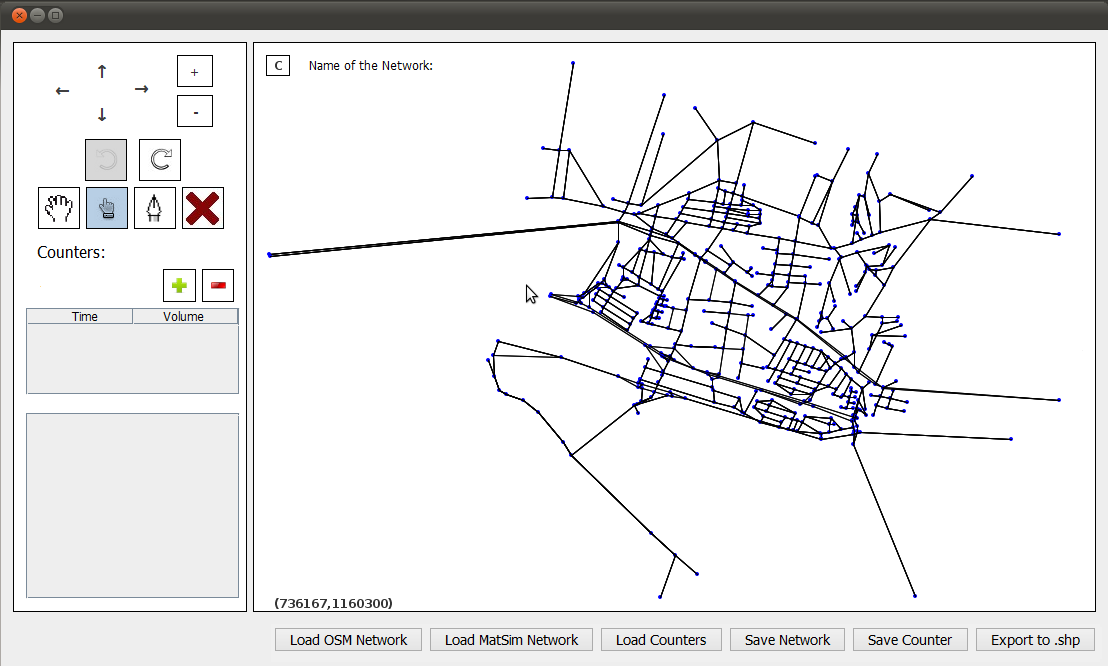
\includegraphics[width=0.99\textwidth, angle=0]{./scenarios/figures/caracasA.png}}%
{}
 %------------

Figure \ref{fig:caracasBleft} shows an image output of the same area after running a simulation generated with \gls{matsim} and including a vehicle-density color map. Figure Figure \ref{fig:caracasBright} shows a sample score graph from one of the many tests run: \textit{avg. trip time} of 02h:06m:38s and \emph{avg. distance per agent} of 1727.83\,meters; \textit{total run time} of the simulation was 41\,minutes 56\,seconds.

 %------------
\createfigure%
{Simulation results.}%
{Simulation results.}%
{\label{fig:caracasB}}%
{%
 \createsubfigure%
 {A snapshot of the area at 7:00\,am  with a color map for vehicle flow.}
 {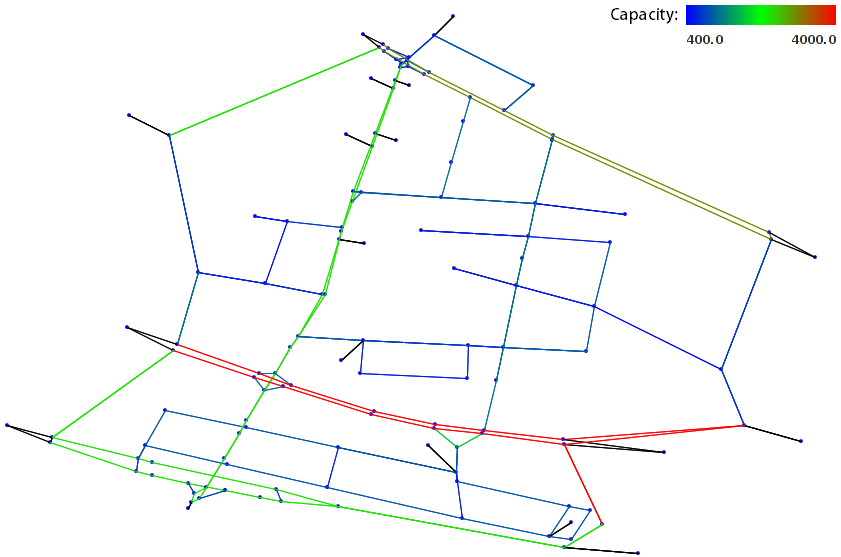
\includegraphics[width=0.49\textwidth, angle=0]{./scenarios/figures/caracasB1.png}}
 {\label{fig:caracasBleft}}
\createsubfigure%
 {\gls{matsim} sample score statistic for one of the scenarios defined.}
 {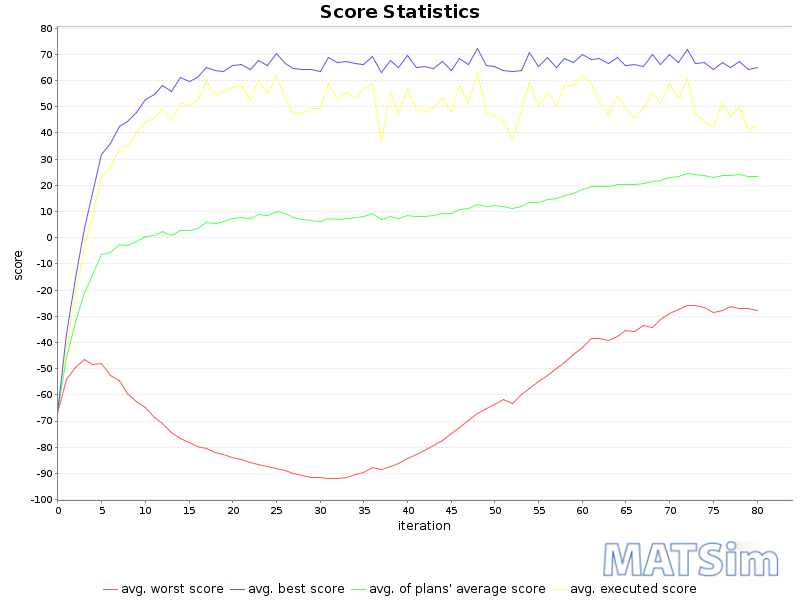
\includegraphics[width=0.49\textwidth, angle=0]{./scenarios/figures/caracasB2.png}}
 {\label{fig:caracasBright}}
}%
{}
 %------------

In spite of the different approaches for generating results between the study made by the company and our own results through simulations, the numbers were quite similar with a range of difference that did not exceed 3\,\% (-0.42\,\% to 2.52\,\%). Taking into account these promising results but also the limitations encountered, the following future lines of work were defined:

\begin{itemize}\styleItemize
\item Run a larger number of simulations to compare with real data to fine tune accuracy of results.

\item The ability to incorporate simulation plans from censuses, polls, among other alternative data sources different from \gls{od}, as well as a methodology that favors the collection of data in a disaggregated fashion.

\item Include more options for the creation of networks. For instance, to create links based on characteristics such as zebra crossings, speed humps, curb extensions and/or a number of traffic signs.

\item Create options to manage a simulation project that incorporates the internal organization made by the tool, where all iterations of simulations are kept separate in folders with all the outputs produced. This also implies the creation of a more refined reporting tool that could be used to support the decision making process of smart traffic devices, contraflow lanes, etc.
\end{itemize}


\paragraph{Acknowledgements}
The authors wish to acknowledge Daniel Ampuero Anca and Jesús Francisco Gómez Ortíz, for their Bachelor's degree final work at \emph{Universidad Central de Venezuela}. Also to Óscar Anzola, founder of \emph{URVISA S.A.}, who provided the logistics for the capture of real traffic data used on the simulations.

% ##################################################################################################################